\documentclass[../main-v1.tex]{subfiles}
\begin{document}
\chapter{Resource Needs Summary}
\label{ch:resource}

\section{Hardware resources}
Chapter \ref{ch:est} described the projected compute and storage needs through 2040, many of which are being met through collaboration contributions. Chapter \ref{ch:netw} describes networking. 



\section{Personnel needs}
Building and managing a project of this complexity also requires a large number of personnel.  Figure \ref{fig:resources} shows a timeline for estimated resource needs.   Efforts are currently spread across a large number of highly expert people working part time on DUNE computing, aside from the five dedicated DOE funded postdocs.  We anticipate that these young people will move into leadership roles in computing in the future.  Although the  FTE are close to the number needed, there is some mis-match in skill-sets. In particular, we anticipate needing several person-years of effort on framework development which is not available with the current mix of personnel. 

\begin{dunefigure}
[Development Personnel needs]
{fig:resources}
{Estimated computing infrastructure personnel needs through 2030.  The dark colors show development areas where experts are needed while the lighter colors show operations tasks where non-experts can contribute. The dashed line shows the estimated effort allocated to the project.  The bump from 2022-2024 is from a 3-year DOE grant.}
{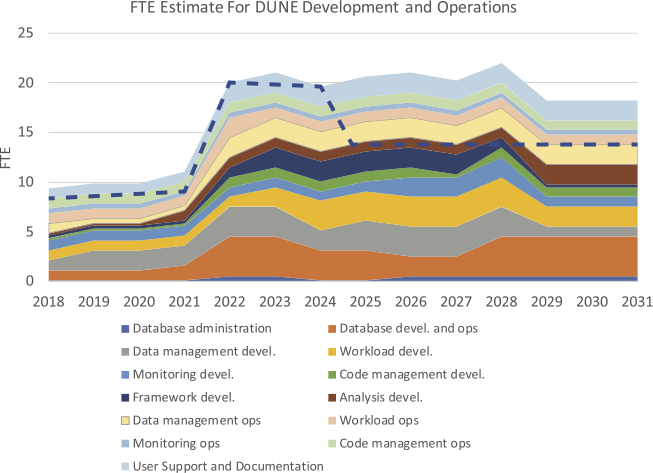
\includegraphics[width=0.9 \textwidth]{graphics/Resources/DetailNeeds-2022-02.xlsx.png}}
\end{dunefigure}

\section{Summary}

This document has described most aspects of \dword{dune} offline computing. Our computing model relies on significant contributions across the collaboration.  

%\hideme{Remove this chapter}
%%%%%%%%%%%%%%%%%%%%%%%%%%%%%%%
%\section{xyz}
%\label{sec:org:xyz}  %% fix label according to section
\end{document}
